\subsection{Dataset Description}

For this study, we collected data from 3 major movies releases of the years 2018 and 2019: Avengers Infinite War, Aquaman, and Captain Marvel. The data gathering process occurred during the debut week of each movie, as showed in Table \ref{tab:range_data}. We collected data from Twitter and YouTube platforms, using their officials APIs. Among the data collected, we selected fields such as [lista de campos] to construct our dataset.  
%The dataset's we used for our evaluation is about the movies: Avengers Infinite War, Aquaman and Captain Marvel, gathered from Twitter and Youtube comments, available on both API's. Among the resources available in sources, we highlight the text (tweet or comment), date timezone, geolocation and retweets/likes. The data gathering process occurred during the debut week of each movie, as following the table \ref{tab:range_data}. 

\begin{table}[h]
    \small{}
    \begin{tabular}{ p{4cm}|p{1.5cm}|p{1.5cm} }
        \hline
            \textbf{Movie} & \textbf{Start} & \textbf{Final}\\
        \hline
            Avengers Infinite War & 04/20/2018  & 05/04/2018 \\
            Aquaman & 12/03/2018 & 12/17/2018  \\
            Captain Marvel & 03/10/2019 & 03/18/2019 \\
        \hline
    \end{tabular}
    \caption{Range of Data Collection}
    \label{tab:range_data}
\end{table}
    
\subsection{Unsupervised Lexicon-Based}

%JS Ajustes AINDA

Sentimental analysis, also known as opinion mining, is a sub-field of Natural Language Processing (NLP). The main purpose of Sentiment Analysis is to identify and extract opinions from a particular text~\cite{vader}. Several approaches have already been developed to identify sentiments in texts. But, generally, those approaches depend on previous annotated data. This was not the case for this study, and so we needed to develop mechanisms to overcome this difficulty. To overwhelm the annotated data problem, we resorted to unsupervised learning techniques. Those techniques use ontologies, databases, and lexicons with detailed information about the specific activity.
% In those situations, we need discover another ways to classified this data. Unsupervised Techniques for predicting the sentiment by using ontologies, databases, and lexicons that have detailed information to specific activity are recommend options. 
%Sentimental analysis, also known as opinion mining, is a sub-field of Natural Language Processing (NLP).It's main goal is to identify and extract opinions from a particular text \cite{vader}. There are many approach's to apply sentiment analysis in texts, but when we hadn't labeled training data to learn patterns, that can be a issue. In those situations, we need discover another ways to classified this data. Unsupervised Techniques for predicting the sentiment by using ontologies, databases, and lexicons that have detailed information to specific activity are recommend options. 

The term lexicon is used to refer to a dictionary or vocabulary with characteristics like a list of positive and negative words with an associated score, and use of techniques like word position, surrounding words, context analysis, part-of-speech, phrases, and others. Various lexicons are used for this analysis, including: AFINN Lexicon, Bing Liu's Lexicon, MPQA subjectivity Lexicon, SentiWordNet, Vader Lexicon, Pattern Lexicon. In the next section will be discuss the Vader Lexicon, chosen for that research. 

%As mentioned, a lexicon is a dictionary or vocabulary, that have a list of positive and negative polar words with some score associate, and using some techniques like the position of words, surrounding words, context, part-of-speech, phrases and etc \cite{Dipanjan:2016}. Various lexicons are used for this analysis, including: AFINN Lexicon, Bing Liu's Lexicon, MPQA subjectivity Lexicon, SentiWordNet, Vader Lexicon, Pattern Lexicon. In the next section will be discuss the Vader Lexicon, chosen for that research. 

\begin{figure*}[t!]
    \begin{center}
    \subfloat[Avengers Infinite War]{{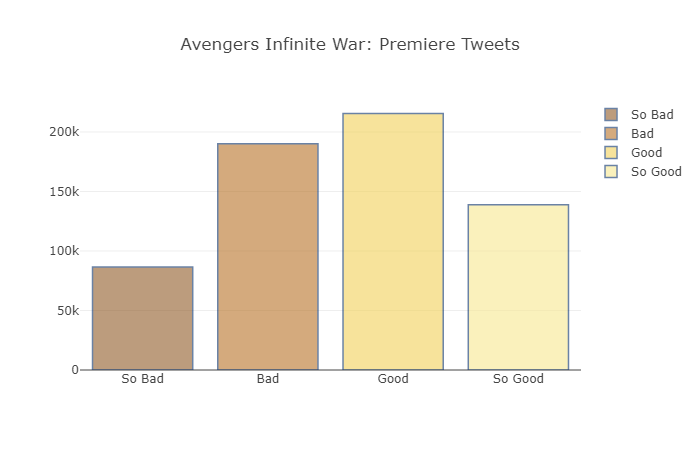
\includegraphics[width=5cm]{img/avengers.png} }}%
    \qquad
    \subfloat[Aquaman]{{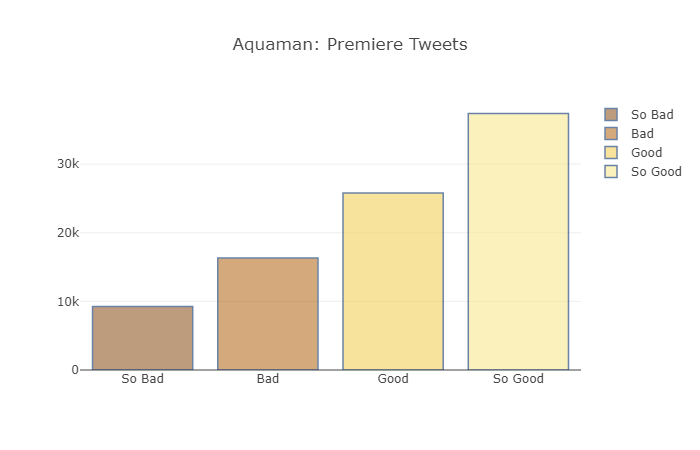
\includegraphics[width=5cm]{img/aquaman.png} }}%
    \qquad
    \subfloat[Captain Marvel]{{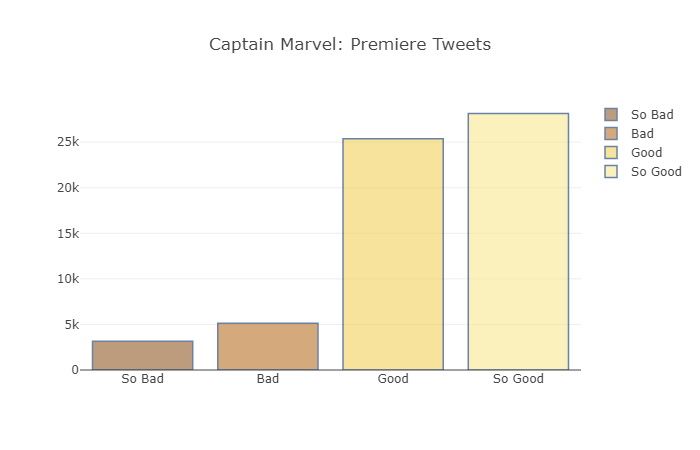
\includegraphics[width=5cm]{img/captain.png} }}%
    \caption{Sentiment Analysis results on the tweets of each movie.}%
    \label{fig:example}%
    \end{center}
\end{figure*}

\subsection{Vader\label{vader}}
%Ver vitor text ou words
Vader (Valence Aware Dictionary and sEntiment Reasoner) Lexicon is a lexicon based on sentiment-related words. In this approach, each word is labeled according to their semantic orientation as either positive or negative. Vader produces 4 sentiments metrics: the first three (positive, negative and neutral) represent the proportion of the words that matching into ant categories. The final metric, \textit{compound} score, is a combination of the first three metrics normalized. The compound score revolves between -1 and 1, where -1 represents highly negative opinion and 1 highly positive opinion.

%Vader (Valence Aware Dictionary and sEntiment Reasoner) Lexicon is based on lexicon of sentiment-related words. In this approach, each words in the context are generally labeled according to their semantic orientation as either positive or negative. Vader produces 4 sentiments metrics: the first three, positive, negative and neutral, represent the proportion of the texts that matching into ant categories. The final metric, \textit{compound} score, is the sum of first three normalized metrics, between -1 and 1, that -1 represents highly negative and 1 highly positive.

%JS review
Since Vader deals with certain features that most of the others lexicon do not (such as Abbreviations, Upper Case, Emojis, and Special characters), it is considered a very appropriate lexicon to be used in Social Media texts evaluation. On the following example, we demonstrate the advantages of using Vader lexicon in Social Media: 

%We consider using Vader Lexicon, to evaluate the tweets texts, for supporting the following aspects that non-normalized text may contain: Abbreviations, Upper Case, Emojis, Special characters. To understand, how Vader is great alternative to text analysis, follow a example: 

\begin{figure}[h]
    \begin{center}
        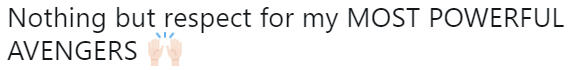
\includegraphics[width=0.8\linewidth]{img/Twitter1.png}
    \end{center}
       \caption{Example tweet using Vader Lexicon.}
    \label{fig:tweet1}
\end{figure}

The \textit{tweet} presented on Figure \ref{fig:tweet1} was evaluated with the following scores for sentiment analysis: \textit{'compound'}: 0.6133, \textit{'neg'}: 0.169, \textit{'neu'}: 0.508, \textit{'pos'}: 0.322. As we can see, the overall evaluation of the text denotes a positive emotion. But if this same text was parsed without considering \textit{emojis} and capital letters, the scores evaluation would be: \textit{'compound'}: 0.2043, \textit{'neg'}: 0.202, \textit{'neu'}: 0.546, \textit{'pos'}: 0.251. In this case, we can notice a significant drop on the \textit{compoud} value, which makes the text's emotion to be classified almost as neutral, instead of positive as it should. 

%The \textit{tweet} shown on Figure \ref{fig:tweet1} presented the following values for the sentiment analysis, \textit{'compound'}: 0.6133, \textit{'neg'}: 0.169, \textit{'neu'}: 0.508, \textit{'pos'}: 0.322, denoting a general positive evaluation (\textit{'compound'}: 0.6133). If the \textit{tweet} was parsed without \textit{emojis} and capital letters were not taken, the values obtained in the evaluation would be: \textit{'compound'}: 0.2043, \textit{'neg'}: 0.202, \textit{'neu'}: 0.546, \textit{'pos'}: 0.251. As we can see, the general evaluation of \textit{tweet} (\textit{compound}) dropped to 0,2043, which, although still a positive value, is closer to the neutral than previously obtained. 

\subsection{TF-IDF\label{TFID}}

\textit{Term Frequency-Inverse Document Frequency} indicates the weigh of text's terms according to its frequency proportion~\cite{Dipanjan:2016}. This technique was developed to be a classification metric for searching users' queries results on search engines.

%Term Frequency-Inverse Document Frequency, which indicates the weighting of terms occurring in texts, in proportion your frequency \cite{Dipanjan:2016}. This technique was developed as classification metric, in search results in search engines, based on user queries. 
\begin{equation*}
    W_{t,d} = \left ( \frac{Freq_{t,d}}{Max} \right ) * log_2 \left ( \frac{N}{n_t} \right)
\end{equation*}

\( W_{t,d}\) represents the term weight \textit{t} in document \textit{d}. \( Freq_{t,d}\) is the number of times that the terms/words occur in text. \( Max\) is the term with the highest number of occurrences in the text. 
%JS Rever!!! Vitor
\( N \) is the total of texts in the base of tests, \( n_t \) is the number of texts in the base of tests that owns the term \( t \).

%\subsection{Approach Proposed}

\subsection{Proposed Approach}

This section will discuss our research approach, described in Figure~\ref{fig:approach}. 
We divided our research into 4 steps. The first step performed was collecting data from Social Media. On this step, we gathered data from both YouTube and Twitter Social Media, using their officials APIs. From Twitter, we collected the tweets' texts, and from YouTube, we collected the users' comments.

After the data gathering step, we needed to pre-processed our data. During this step, we removed the texts' links, distributed the data in a temporal series, and tokenize the text. We did not remove the stopwords because Vader Lexicon uses them on the evaluation process.

%This section will discuss the research approach proposed, describe in the Figure \ref{fig:approach}. The first step taken is extracting data from social media API's. Text from tweets and youtube's comments are collected, then preprocessing is performed in collection data, including separation of the data in a serie temporal, according to the premiere date, tokenzation and removal links. The stopwords process will not considered in the model, because it acts negatively on the results obtained from Vader Lexicon.

On the third step, we used Vader to perform Sentiment Analysis on our texts. This analysis provided us the sentiment scores and compound values (see section \ref{vader}) for the Tweets and comments collected. The texts were then split into several files, according to their polarity. 
%Next, we performed Vader Lexicon to get the Sentiment Score and Compound (mentioned in section \ref{vader}), and after, we realized the data separation in files, according to its polarity. In Data Analysis process, we already have the polarity of each text (sentence), then we calculate TF-IDF in created files, that we know about the important frequency terms in the whole document.

The last step of our study was the Data Analysis. On this step, we calculated the TF-IDF (see section \ref{TFID}) statistics on the files generated on the previous step. These statistics provided us information about the most frequent and relevant terms on the documents. 
%In Data Analysis process, we already have the polarity of each text (sentence), then we calculate TF-IDF in created files, that we know about the important frequency terms in the whole document.

%To establishing a textual standard, through Pos-Tag (Part-of-Speach) feature, we find for the terms classified as adjectives, within the results from most frequency terms, thus allowing the texts recommendation creation to each movie. 

\begin{figure*}[h]
\begin{center}
% \fbox{\rule{0pt}{2in} \rule{.9\linewidth}{0pt}}
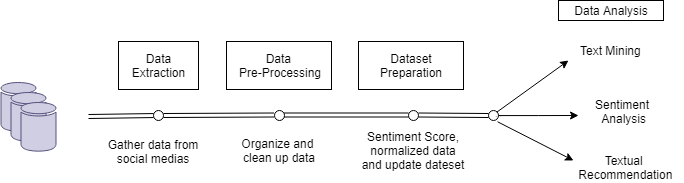
\includegraphics[width=0.6\linewidth]{img/model.png}
\end{center}
   \caption{Approach overview: Sentiment analysis of the Blockbluster Movies 2018-2019.}
\label{fig:approach}
\end{figure*}

\subsection{Tweets behaviour about movies}

\subsection{Textual recommendation}

In this step, the use's TF-IDF features is necessary, to evaluate how important a term/word in a given document\cite{Dipanjan:2016}. From the results obtained by the lexicons, we divided in files, according with texts polarity, to calculate the TF-IDF. Therefore, we will have the most used terms in negative and positive texts. 

From the most used terms found in the texts, we proceed to the identification the lexical category in which the words are assigned based on their syntactic context and role, called POS (Part-of-Speech) Tagging. Using NLTK Library, which generate outputs specific tags for certain word, we can mention: \textit{Adjectives, Nouns, Adverbs, Coordination Conjuntion, Verbs, Preposition and etc}. 

\begin{verbatim}
    [('ragnarok', 'NN')],256
    [('saying', 'VBG')],2152
    [('rich', 'JJ')],125
    [('lots', 'NNS')],102
    [('much', 'JJ')],3509
\end{verbatim}

{\renewcommand\arraystretch{1.25}
\begin{tabular}{|c|c|c|}

    \hline
        \multirow{3}{*}{Avengers} & 
            \multicolumn{2}{p{6cm}|}{\raggedright Avengers was \textit{greatest, biggest, best} movie have I saw.} & 
            \cline{2-3} & 
            \multicolumn{2}{p{6cm}|}{\raggedright Avengers made me \textit{angry, depressed, worried, and physically weak} with the scene final.} & 
    \hline
        \multirow{3}{*}{Aquaman} & 
            \multicolumn{2}{p{6cm}|}{\raggedright Aquaman \textit{impressed} (\textit{surprised}) me \textit{positively}, with \textit{incredibles} visual effects. DC Comics has built a great, fantastic and solid movie for all fans.} & 
            \cline{2-3} & 
            \multicolumn{2}{p{6cm}|}{\raggedright Avengers was \textit{greatest, biggest, best} movie have I saw.} & 
    \hline
        \multirow{3}{*}{Captain M.} & 
            \multicolumn{2}{p{6cm}|}{\raggedright Avengers was \textit{greatest, biggest, best} movie have I saw.} & 
            \cline{2-3} & 
            \multicolumn{2}{p{6cm}|}{\raggedright Avengers was \textit{greatest, biggest, best} movie have I saw.movie have I saw.movie have I saw.} & 
    \hline
\end{tabular}

